\documentclass[a4paper, 11pt]{article}
\usepackage{comment} % enables the use of multi-line comments (\ifx \fi) 
\usepackage{lipsum} %This package just generates Lorem Ipsum filler text. 
\usepackage{fullpage} % changes the margin
\usepackage{graphicx, wrapfig, subcaption, setspace, booktabs}
\usepackage{url}

\begin{document}
%Header-Make sure you update this information!!!!
\noindent
\large\textbf{Exploring delays in air travel in the United States} \hfill \textbf{Sara Arango-Franco} \\
\normalsize \url{github.com/sarangof/air-travel-USA/} 

\section*{Problem Statement}
The RITA data set (from the Office of the Assistant Secretary for Research and Technology of the Department of Transportation) consists on records of airplane trips between airports in the United States since 1987. In this exercise I wondered about flight delays: how do they distribute geographically? What are the most important airports in the country in terms of connections? What are the most "vulnerable" in the sense of the ratio between importance and high rates of delays?

A conversation with an airline schedule specialist made me wonder if it is true that carriers are extending scheduled flight duration in order to have a better on-time performance. I aggregated the data sets in a way that shows that the average schedule duration is, in effect, increasing, but the on-time performance is not necessarily improving.

\section*{Airports as a network}


I represented airports in the data set \footnote{Used 2008 data because it was the most recent year in the source that I ended up acquiring the data from.} as nodes in a network, where the edges are the presence of direct flights between those airports, and the weights are the total number of trips between airports in a year. Used \textit{betweenness centrality} as a measure of the importance of each airport in terms of incoming and outgoing \textit{domestic} connections. The top ten airports according to this ranging are listed in Table \ref{centrality}. Notice that these airports are not necessarily the largest or busiest terminals in the United States. A proof of this is that airports with higher local relevance become more important, whereas big airports with large flux of international flows, such as JFK, lose focus.


\captionof{table}{Top 10 most important airports in terms of betweenness centrality.}
\resizebox{5 cm}{!}{
\centering
\begin{tabular}{|l c|}
\centering
\label{centrality}
%\hline
\textbf{Airport} & \textbf{ArrDelay} \\
\hline
Atlanta &	0.133890 \\
Dallas 	& 0.085455 \\
Salt Lake City & 	0.084728 \\
Minneapolis  &	0.082088 \\
Anchorage & 	0.058786 \\
Chicago 	& 0.056784 \\
Denver 	& 0.051072 \\
Detroit 	& 0.042831 \\
Houston 	& 0.040318 \\
San Francisco & 	0.038127 \\
%\hline
\end{tabular}
}

\vspace*{0.5cm}

When wanting to know about the performance of the airports (nodes) in this network, I identified the worst performing airports in terms of delays \footnote{This is a big assertion to make because the system itself is complex and airlines, weather and other factors impact performance. But, with a sufficiently large amount of data points -like our case- trends can be seen and studied.}. The list of airports that present the worst arrivals in arrival performance are listed in Table \ref{arrival_performance}. A rank is also presented for departure performance in Table \ref{departure_performance}.


\captionof{table}{Worst performing airports in terms of arrival performance.}
\resizebox{5 cm}{!}{
\centering
\begin{tabular}{|l c|}
\centering
\label{arrival_performance}
%\hline
\textbf{destin city} & \textbf{ArrDelay} \\
\hline
Springfield 	& 63.447158 \\
Aspen 	& 29.995056 \\
Gunnison  &	28.909466 \\
Nantucket &	26.079958 \\
Des Moines &  	24.121120 \\
North Bend 	& 20.736623 \\
Norfolk 	& 20.653845 \\
Chico 	& 19.905077 \\
Eagle 	& 19.462659 \\
Butte 	& 18.991971 \\
%\hline
\end{tabular}
}
\vspace*{0.5cm}


\captionof{table}{Worst performing airports in terms of departure performance.}
\resizebox{5 cm}{!}{
\centering
\begin{tabular}{|l c|}
\centering
\label{departure_performance}
%\hline
\textbf{origin city} &	\textbf{DepDelay} \\
Champaign &	149.266698 \\
Roanoke 	& 51.956570 \\
Arcata/Eureka & 	48.000720 \\
Klamath Falls &	47.066221 \\
Wichita 	& 39.904703 \\
Appleton &	36.742313 \\
Charlottesville & 	32.597403 \\
Grand Junction & 	31.171125 \\
Fargo 	& 30.783061 \\
Nantucket 	& 29.892045 \\
%\hline
\end{tabular}
}
\vspace*{0.5cm}

Although this is important to know, most of the airports in these lists are small and are not very relevant in the system itself. That is why I decided to create a ratio of bad performance relative to network importance for domestic flights. This \textit{index} is calculated as follows:

$$Vulnerability_{airport}=\frac{Average\_delay_{airport}}{Centrality_{airport}}$$

The most "vulnerable" airports in terms of arrivals are listed in Table \ref{vul_arrivals} and plotted in Figure \ref{arr_plot}. The same list is presented for departures in Table \ref{vul_departues} and mapped in Figure \ref{dep_plot}.

\captionof{table}{Most vulnerable airports (arrival).}
\resizebox{5 cm}{!}{
\centering
\begin{tabular}{|l c|}
\centering
\label{vul_arrivals}
%\hline
\textbf{destin city }& \textbf{	ind} 	 \\
Atlanta 	& 0.160344 	 \\
Salt Lake City & 	0.128662 	\\
Minneapolis 	& 0.127824 	 \\
Dallas 	& 0.126783 	 \\
Detroit 	& 0.101268 	 \\
Denver 	& 0.076429 	 \\
Chicago 	& 0.062064 	\\
Houston 	& 0.059642 	\\
Anchorage &	0.057610 \\	
Phoenix 	& 0.055963 	\\

%\hline
\end{tabular}
}








\begin{figure}[!ht]
  \caption{Arrival vulnerability (continental USA).}
  \label{arr_plot}
  \centering
    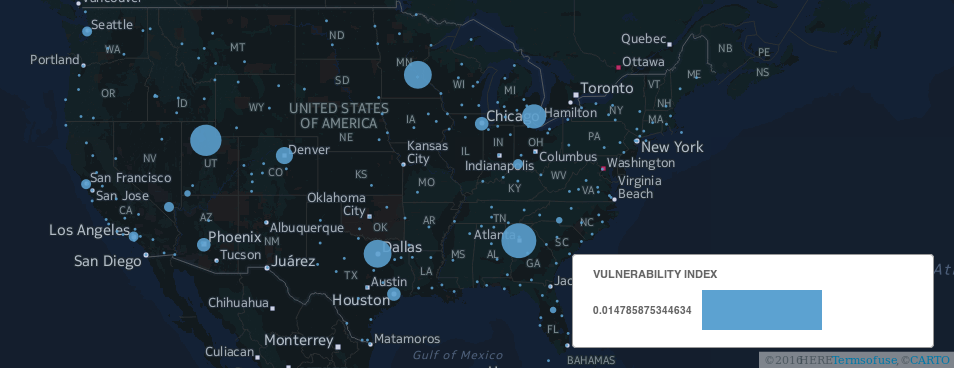
\includegraphics[width=\textwidth]{/home/saf537/Documents/Spotify/air-travel-USA/plots/arrival_vulnerability}
\end{figure}



\captionof{table}{Most vulnerable airports (departure).}
\resizebox{5 cm}{!}{
\centering
\begin{tabular}{|l c|}
\centering
\label{vul_departues}
%\hline
\textbf{destin} & \textbf{city 	ind} 	\\
Anchorage & 0.182137 	\\
Atlanta 	& 0.167439 	\\
Salt Lake City & 	0.121132 	\\
Dallas 	& 0.107078 	\\
Minneapolis & 	0.101947 \\	
Chicago 	& 0.084103 	\\
Los Angeles  &	0.083590 \\	
Seattle  &	0.072145 	\\
San Francisco & 	0.065996 	\\
Denver &	 0.062989 	\\

%\hline
\end{tabular}
}



\begin{figure}[!ht]
  \caption{Departure vulnerability (continental USA).}
  \label{dep_plot}
  \centering
    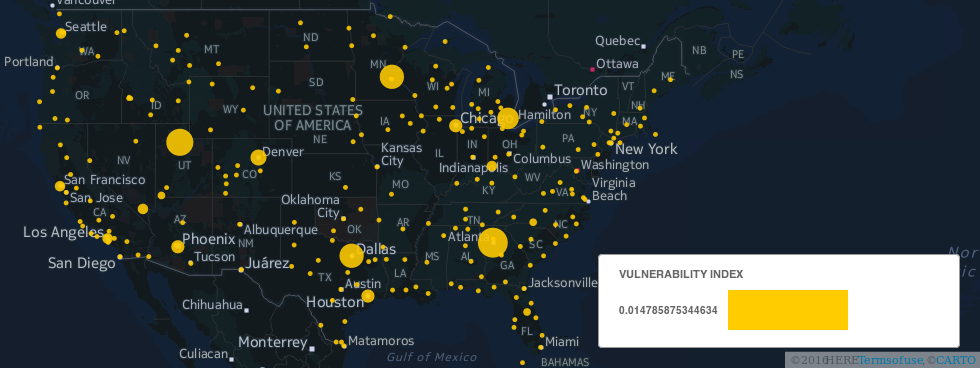
\includegraphics[width=\textwidth]{/home/saf537/Documents/Spotify/air-travel-USA/plots/departure_vulnerability}
\end{figure}


Airports like San Francisco's SFO lose focus as, although they are important in terms of connections, they have better performance in terms of delays, whereas airports like Alaska's Ted Stevens airport in Anchorage become more important for their relative importance in the network compared to their performance. 

The proposed index displays which nodes are more sensitive in the domestic flights network, and thus need more attention. It is important to notice that international flights are excluded from this analysis, introducing a significant bias.


%\begin{figure}[!ht]
%  \caption{Missing days in the dataset.}
%  \label{m_days}
%  \centering
%    \includegraphics[scale=0.6]{/home/saf537/Documents/Spotify/air-travel-USA/plots/test}
%\end{figure}

\section*{Is on-time performance improving with time?}

A conversation with an airline industry engineer made me suspect that it may be the case that airlines increase the scheduled flight duration in order to improve their performance metrics. In order to test this hypothesis I used aggregated flight data from 1987 to 2008. It is worth noting that an important amount of data cleaning in processing was needed to be performed before any comparison, because of the following reasons:

\begin{itemize}
\item Routes were closed or non consistent along the years. Those routes were deleted from the data set.
\item A simple average on the trip length in each year is misleading and incorrect. Instead, trip length was aggregated and averaged between same origin-destination pairs, and further aggregated and averaged over each year. This guarantees that only comparable trip lengths were actually compared.
\end{itemize}


Figure \ref{schedule} shows an increasing trend in the average length of trips. A linear regression shows that this trend is significantly increasing \footnote{P-value of $1.078e-08$ and $R^2$ of $0.94$.}
Schedule. Despite of this, Figure \ref{delays} does not show a clear trend on arrival performance, which is confirmed by poor performance of the statistical test in a linear regression \footnote{P-value: $0.414$. $R^2$: $0.212$.}. 



\begin{figure}[!ht]
  \caption{Scheduled trips length along the years in question.}
  \label{schedule}
  \centering
    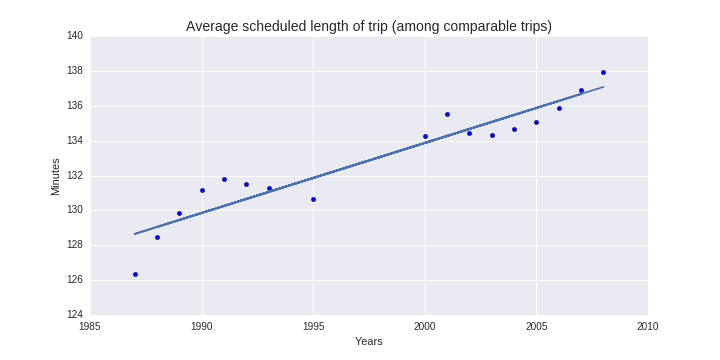
\includegraphics[width=\textwidth]{/home/saf537/Documents/Spotify/air-travel-USA/plots/schtrips}
\end{figure}

\begin{figure}[!ht]
  \caption{Total delay along the years in question.}
  \label{delays}
  \centering
    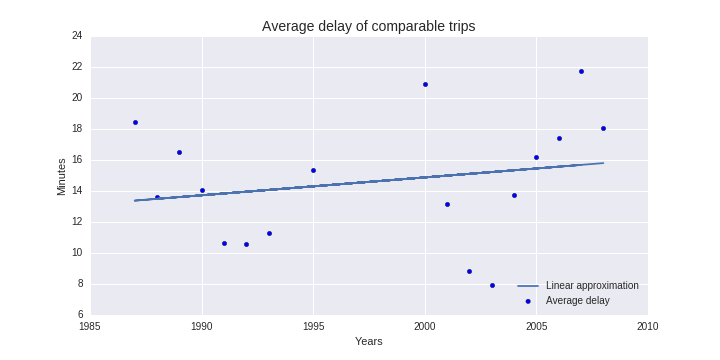
\includegraphics[width=\textwidth]{/home/saf537/Documents/Spotify/air-travel-USA/plots/deltrips}
\end{figure}

It is worth noting that causality was not investigated in this exercise.

\section*{Comments and conclusions}

\begin{itemize}
\item A simple index was created to indicate which airports deserve more attention in terms of their relative importance in the domestic flight network given their delay performance.
\item A test was performed in order to investigate whether performance has improved, and whether flights are scheduled with longer buffer times.
\end{itemize}

% to comment sections out, use the command \ifx and \fi. Use this technique when writing your pre lab. For example, to comment something out I would do:
%  \ifx
%	\begin{itemize}
%		\item item1
%		\item item2
%	\end{itemize}	
%  \fi




\end{document}
